% Author: Dun-Ming Huang
% Email: dunmingbrandonhuang@berkeley.edu
% CSM16A Fall 2022

\qns{Yes Cap}

\textbf{Learning Goal}: Learn of the fundamentals of capacitors and equivalent capacitance.

\meta{
    \begin{bindenum}
        \item Generally, the \textbf{most efficient method of going through these subparts is to introduce the general formula} before attempting to answer. (The subpart more or less guides the students onto such direction)
    \end{bindenum}
}

Capacitor Sword Man is one of the most well known brand for selling swords in the galaxy. Recently, they have came to Earth on a field trip, and picked up some almost broken capacitors and resistors form the floor of Cory Hall to experiment new lightsaber switches. \\
Cap Sword Man (CSM) has now appeared in your dream to ask you about capacitors.

\begin{enumerate}
    \item {
        Let us first look at this structure:
        \begin{center}
            % Author: Dun-Ming Huang
% Email: dunmingbrandonhuang@berkeley.edu
% CSM16A Fall 2022

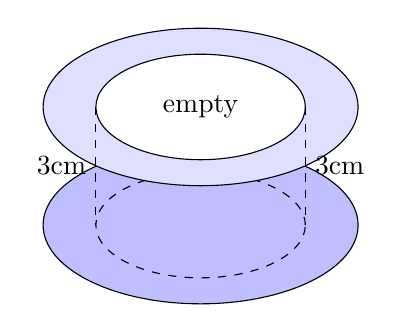
\begin{tikzpicture}
    \draw[fill=blue!50!white!50!] (0,0) ellipse (2cm and 1cm);
    \draw[dashed] (0,0) ellipse (1.33cm and 0.67cm);
    \draw[fill=blue!50!white!25!] (0,1.5) ellipse (2cm and 1cm);
    \draw[fill=white!50!] (0,1.5) ellipse (1.33cm and 0.67cm) node{empty};
    \draw[dashed] (1.33, 1.5) -- (1.33, 0) node[midway, right]{3cm};
    \draw[dashed] (-1.33, 1.5) -- (-1.33, 0) node[midway, left]{3cm};
\end{tikzpicture}
        \end{center}
        The colored rings and circles are conductor plates, each with an outer radius of 4cm. Meanwhile, the top conductor plate is a ring whose inner radius is 3cm. \\
        The permittivity of the material they put between the conductor ring and the conductor plate is $10 F/m$. \\
        The vertical distance between the ring and the plate is 3 cm.
        What is the capacitance of this capacitor CSM just built?
        
    }
    \meta{
        Be careful about the \textbf{higher conducting ring having an empty section}. Students might miss it.
        
    }
    \ans{
        Recall that the capacitance of a capacitor can be calculated as:
        \[C = \frac{\epsilon A}{d}\]
        Such that $\epsilon$ is the permittivity of material between the conducting plates, $A$ is the overlapping area of the conducting plates (Which is the origin of the charge-storing electric fields), and $d$ is the distance between conducting plates. \\
        Therefore, using the provided statistic of the problem:
        \begin{align*}
            C &= \frac{10 F/m \times (4^2 \pi - 3^2 \pi) {cm}^2}{3cm} \\
            &= \frac{10 \times 0.0007\pi m^2}{0.03 m} = 0.73F
        \end{align*}
    
    }
    
    \item {
        CSM has decided to just use the capacitors they picked up from Cory Floor instead, but they only picked up $1mF$ capacitors. They now use the knowledge of resistors and attempt to see if the following combination produces a capacitor whose equivalent capacitance is different from $1mF$:
        \begin{center}
            % Author: Dun-Ming Huang
% Email: dunmingbrandonhuang@berkeley.edu
% CSM16A Fall 2022

\begin{circuitikz}[american]
    \draw
        (0, 0)
        to[short, o-] (1, 0)
        to [C, l^=$1mF$] (2, 0)
        to [C, l^=$1mF$] (3, 0)
        to [short, -o] (4, 0);
\end{circuitikz}
        \end{center}
        Calculate the equivalent capacitance, and \textbf{in addition}, derive the capacitance formula for capacitors in series.
    
    }
    \ans{
        Mind that when in series, all capacitors have the same current flowing across it. \\
        Therefore, using this configuration as the base of discussion:
        \begin{center}
            % Author: Dun-Ming Huang
% Email: dunmingbrandonhuang@berkeley.edu
% CSM16A Fall 2022

\begin{circuitikz}[american]
    \draw
        (0, 0)
        to[short, o-] (1, 0)
        to [C, l^=$C_1$, i_=$i_1$] (2, 0)
        to [C, l^=$C_2$, i_=$i_2$] (3, 0)
        to [short, -o] (4, 0);
\end{circuitikz}
        \end{center}
        via KCL, we first attain $i_1 = i_2$. \\
        Therefore, provided that for each capacitor, $I_c = C \pdv{V_C}{t}$, we may dictate what follows:
        \begin{align*}
            \Sigma V &= V_1 + V_2 \\
            \pdv{\Sigma V_C}{t} &= \pdv{V_{C_1}}{t} + \pdv{V_{C_2}}{t} \\
            I_c &= \Sigma C \pdv{\Sigma V_{C}}{t} \\
            &= C_1 \pdv{V_{C_1}}{t} = C_2 \pdv{V_{C_2}}{t} \\
            \frac{I_c}{C_1} + \frac{I_c}{C_2} &= \pdv{\Sigma V_C}{t} \\
            I_c &= \frac{1}{ \frac{1}{C_1} + \frac{1}{C_2} } \pdv{\Sigma V_C}{t} \\
            \Sigma C &= \frac{1}{ \frac{1}{C_1} + \frac{1}{C_2} }
        \end{align*}
        Utilizing the above formula as we substitute each capacitance with $1mF$, we attain the situation that CSM attempts to inspect, and find that the equivalent capacitance of the prompt's configuration is $2mF$.
    
    }
    
    \item {
        CSM is satisfied with your answer. Then, CSM continues to use the knowledge of resistors, and attempt to see the equivalent capacitance and potential energy that the following configuration produces:
        \begin{center}
            % Author: Dun-Ming Huang
% Email: dunmingbrandonhuang@berkeley.edu
% CSM16A Fall 2022

\begin{circuitikz}[american]
    \draw
        (-1.5, 0) node[ground]{}
        to [V, l^=$5V$, invert] (0, 0)
        to [C, l^=$1mF$] (1, 0)
        to [short] (1, 1)
        to [C, l^=$1mF$] (2, 1)
        to [short] (2, 0)
        to [short] (3, 0) node[ground]{}
        (1, 0)
        to [short] (1, -1)
        to [C, l^=$1mF$] (2, -1)
        to [short] (2, 0);
\end{circuitikz}
        \end{center}
        Calculate the energy of capacitors for them.
        
    }
    \ans{
        Let us first figure out how does equivalent capacitance of parallel capacitors work, by discussing the following configuration:
        \begin{center}
            % Author: Dun-Ming Huang
% Email: dunmingbrandonhuang@berkeley.edu
% CSM16A Fall 2022

\begin{circuitikz}[american]
    \draw
        (0, 0) node[ground]{}
        to [short] (1, 0)
        to [short] (1, 1)
        to [C, l^=$C_1$, i_=$i_1$] (2, 1)
        to [short] (2, 0)
        to [short] (3, 0) node[ground]{}
        (1, 0)
        to [short] (1, -1)
        to [C, l^=$C_2$, i_=$i_2$] (2, -1)
        to [short] (2, 0);
\end{circuitikz}
        \end{center}
        In this case, due to the parallel nature of circuit, $V_{C_1} = V_{C_2}$. Therefore, $\pdv{\Sigma V}{t} = \pdv{V_{C_1}}{t} = \pdv{V_{C_2}}{t}$\\
        Meanwhile, the current passing through the overall combination of capacitors can be computed via KCL as $i_1 + i_2$. \\
        Therefore, we attain that:
        \begin{align*}
            \Sigma C \pdv{\Sigma V}{t} &= i_1 + i_2 \\
            &= C_1 \pdv{V_{C_1}}{t} + C_2 \pdv{V_{C_2}}{t} \\
            &= (C_1 + C_2) \pdv{\Sigma V}{t} \\
            \Sigma C &= C_1 + C_2
        \end{align*}
        for the parallel capacitor. \\
        Then, the equivalent capacitance of the prompt's configuration (a $1mF$ and a $2mF$ in series) is in fact:
        \[\frac{1}{\frac{1}{1mF} + \frac{1}{2mF}} = 0.67mF\]
        The overall capacitor potential energy is therefore:
        \[\Sigma E = \frac{1}{2} \Sigma C V^2 = 0.5 \times 0.67mF \times 25V^2 = 8.375mJ\]
        
    }
    
    \item {
        CSM notices from your lecture notes that there is something called ``superposition''. He also noticed that he only has two voltage sources, both of which are not of the supply he wants; however, its difference is. \\
        Derive the voltage at the marked node ($V_x$) on the circuit, and verify whether superposition works to solve it:
        \begin{center}
            % Author: Dun-Ming Huang
% Email: dunmingbrandonhuang@berkeley.edu
% CSM16A Fall 2022

\begin{circuitikz}[american]
    \draw
        (0, 0) node[ground]{}
        to [V, l^=$V_1$, invert] (0, 3)
        to [C, l_=$1mF$] (1.5, 3) node[circ, fill=black, label=above:$V_x$]{}
        to [C, l_=$1mF$] (3, 3)
        to [V, l^=$V_2$] (3, 0) node[ground]{};
\end{circuitikz}

        \end{center}
    
    }
    \meta{
        \begin{bindenum}
            \item Generally, superposition applies for circuits with voltage sources and capacitors, under the premise that we do not bother calculating power (since power cannot be calculated with superposition due to its nonlinear nature) as well as have independent sources whose supply is constant, and dependent sources have linear supply. What listed above is a strict constraint, for more see: \href{https://en.wikipedia.org/wiki/Superposition_theorem}{here}.
            \item Having multiple voltage sources makes this question weird. Think of capacitors as elements that receive the same amount of current.
        \end{bindenum}
    
    }
    \ans{
        \textit{\textbf{Let $C_1$ generally refer to the left capacitor, and $C_2$ right, in this question.}}
        
        Let us first discuss how the capacitive voltage divider:
        \begin{center}
            % Author: Dun-Ming Huang
% Email: dunmingbrandonhuang@berkeley.edu
% CSM16A Fall 2022

\begin{circuitikz}[american]
    \draw
        (0, 0) node[ground]{}
        to [V, l^=$V$, invert] (0, 3)
        to [C, l_=$C_1$] (1.5, 3) node[circ, fill=black, label=above:$V_x$]{}
        to [C, l_=$C_2$] (3, 3)
        to [short] (3, 0) node[ground]{};
\end{circuitikz}
        \end{center}
        In such a generalized case where the net potential drop across $C_1$ and $C_2$ is $V$, let us name the voltage across $C_1$ as $V_{C_1}$, and that across $C_2$ be $V_{C_2}$. We would realize that:
        \[V = V_{C_1} + V_{C_2}\]
        Since the current across all capacitors is the same and all capacitors start uncharged, the charge across all capacitors is equal in amount. Therefore,
        \[C_1 V_{C_1} = C_2 V_{C_2}\]
        Let us combine the two above clues:
        \begin{align*}
            C_1 V_{C_1} &= C_2 (V - V_{C_1}) \\
            (C_1 + C_2) V_{C_1} &= C_2 V \\
            V_{C_1} &= \frac{C_2 V}{C_1 + C_2} \\
            V_{C_2} &= \frac{C_1 V}{C_1 + C_2}
        \end{align*}
        Let us apply this view to the case presented by the prompt:
        \begin{center}
            % Author: Dun-Ming Huang
% Email: dunmingbrandonhuang@berkeley.edu
% CSM16A Fall 2022

\begin{circuitikz}[american]
    \draw
        (0, 0) node[ground]{}
        to [V, l^=$V_1$, invert] (0, 3)
        to [C, l_=$1mF$] (1.5, 3) node[circ, fill=black, label=above:$V_x$]{}
        to [C, l_=$1mF$] (3, 3)
        to [V, l^=$V_2$] (3, 0) node[ground]{};
\end{circuitikz}

        \end{center}
        In this case, the voltage at node $V_x$ would, however, apply with a different logic since the appearance of two voltage sources is odd. Exploiting that every capacitor has the same charge across:
        \begin{align*}
            C_1 (V_1 - V_x) &= C_2 (V_x - V_2) \\
            C_1 V_1 + C_2 V_2 &= (C_1 + C_2) V_x \\
            V_x &= \frac{C_1 V_1 + C_2 V_2}{C_1 + C_2}
        \end{align*}
        
        Now let us attempt at superposition. Without re-demonstrating the capacitive voltage divider formula:
        \textbf{Keep $V_1$}:
        \begin{center}
            \input{../../topics/capacitors/q_cap_basic_des//cap_supo_v1.tex}
        \end{center}
        \[V_x = \frac{C_1 V_1}{C_1 + C_2}\]
        \textbf{Keep $V_2$}:
        \begin{center}
            \input{../../topics/capacitors/q_cap_basic_des//cap_supo_v2.tex}
        \end{center}
        \[V_x = \frac{C_2 V_2}{C_1 + C_2}\]
        
        At last, combining the above cases, we attain the same sum voltage:
        \[V_x = \frac{C_1 V_1 + C_2 V_2}{C_1 + C_2}\]
        And we would then just substitute both capacitors with $1mF$.
    
    }
    
    \item {
        Now, CSM replaces the $1mF$ capacitor at the right of the above architecture with a custom capacitor that is combined with the lightsaber switch button. Therefore, the capacitor at the right now has a variable capacitance such that for $d$ being the distance that button is pressed into,
        \[C(d) = \frac{{10}^{-3}}{0.1 - d} F\]
        You also have a voltmeter which can return the voltage it reads to a computer. Once the computer chip receive some voltage lower than a specific value, it will turn the switch on and activate the lightsaber. \\
        Now, given the above architecture, find ways to fit the voltmeter and computer chip into the circuit architecture to achieve the above demands, and calculate $V_x$ as a function of $d$.
    
    }
    \ans{
        First of all, using the prior part, we are at least able to determine that:
        \begin{align*}
            V_x &= \frac{C_1 V_1 + C_2 V_2}{C_1 + C_2} \\
            &= \frac{1mF V_1 + \frac{1}{0.1 - d} mF V_2}{1 + \frac{1}{0.1 - d}} \\
            &= \frac{(0.1 - d)mF V_1 + 1 mF V_2}{1.1 - d } \\
        \end{align*}
        Since the voltmeter needs to connect to the node $V_x$ to attain its voltage reading, and need to connect to a computer chip, we can connect the voltmeter in parallel with the rightside capacitor (determined by $C(d)$; meanwhile, a voltmeter is expected to have infinite resistance), and connect the computer chip to that node, then ground the computer chip.
    
    }
\end{enumerate}
